%%%%%%%%%%%%%%%%%%%%%%%%%%%%%%%%%%%%%%%%%%%%%%%%%%%%%%%%%%%%%%%%%%%%%%%%%%%%%%%
% intro.tex: Introduction to the thesis
%%%%%%%%%%%%%%%%%%%%%%%%%%%%%%%%%%%%%%%%%%%%%%%%%%%%%%%%%%%%%%%%%%%%%%%%%%%%%%%%
\chapter{Introduction}
\label{intro_chapter}
%%%%%%%%%%%%%%%%%%%%%%%%%%%%%%%%%%%%%%%%%%%%%%%%%%%%%%%%%%%%%%%%%%%%%%%%%%%%%%%%

\textcolor{red}{This entire chapter is postponed until I have a substantial amount of the data analysis completed and written up. }


%%%%%%%%%%%%%%%%%%%%%%%%%%%%%%%%%%%%%%%%%%%%%%%%%%%%%%%%%%%%%%%%%%%%%%%%%%%%%%%%
% CMB Science {{{
%%%%%%%%%%%%%%%%%%%%%%%%%%%%%%%%%%%%%%%%%%%%%%%%%%%%%%%%%%%%%%%%%%%%%%%%%%%%%%%%
\section{Cosmic Microwave Background Radiation}
\label{sec:cmb_science}
%%%%%%%%%%%%%%%%%%%%%%%%%%%%%%%%%%%%%%%%%%%%%%%%%%%%%%%%%%%%%%%%%%%%%%%%%%%%%%%%

There was a big bang. Some gravity waves were probably generated. They may have left a signature polarization pattern on the \ac{CMB}. 

Measurements of the E-mode polarization (due to things that are not primordial gravity waves) have informed us about the evolution of universe. 
Measurements of B-mode polarization due to primordial gravity waves would tell us about the earliest moments in the history of the universe. (and interesting things like the energy scale of inflation and may confirm or rule out expansion models).
Measurements of B-mode polarization due to other stuff tells us about that other stuff. 

%%%%%%%%%%%%%%%%%%%%%%%%%%%%%%%%%%%%%%%%%%%%%%%%%%%%%%%%%%%%%%%%%%%%%%%%%%%%%}}}

%%%%%%%%%%%%%%%%%%%%%%%%%%%%%%%%%%%%%%%%%%%%%%%%%%%%%%%%%%%%%%%%%%%%%%%%%%%%%%%%
% High-Altitude Ballooning {{{
%%%%%%%%%%%%%%%%%%%%%%%%%%%%%%%%%%%%%%%%%%%%%%%%%%%%%%%%%%%%%%%%%%%%%%%%%%%%%%%%
\section{High-Altitude Ballooning}
\label{sec:balloons}
%%%%%%%%%%%%%%%%%%%%%%%%%%%%%%%%%%%%%%%%%%%%%%%%%%%%%%%%%%%%%%%%%%%%%%%%%%%%%%%%

Explain the motivation for flying a CMB telescope from a high-altitude balloon. 
The advantages. 
The disadvantages. 

Balloons are powerful platforms for achieving low budget and fast (relative to satellites!) astrophysical studies. The high altitude observation environment enables measurement of frequencies inaccessible on the ground ($>$ 350 GHz?). 

\begin{figure}[htbp]
\begin{center}
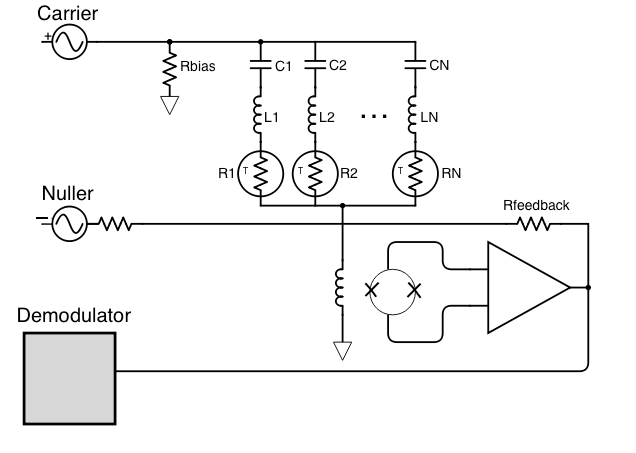
\includegraphics[width=0.6\columnwidth]{figures/dfmux_schematic.png}
\caption{Schematic of readout electronics. 
\label{fig:dfmux} }
\end{center}
\end{figure}



%%%%%%%%%%%%%%%%%%%%%%%%%%%%%%%%%%%%%%%%%%%%%%%%%%%%%%%%%%%%%%%%%%%%%%%%%%%%%}}}



%%%%%%%%%%%%%%%%%%%%%%%%%%%%%%%%%%%%%%%%%%%%%%%%%%%%%%%%%%%%%%%%%%%%%%%%%%%%%%%%
% EBEX {{{
%%%%%%%%%%%%%%%%%%%%%%%%%%%%%%%%%%%%%%%%%%%%%%%%%%%%%%%%%%%%%%%%%%%%%%%%%%%%%%%%
\section{The E and B EXperiment}
\label{sec:ebex}
%%%%%%%%%%%%%%%%%%%%%%%%%%%%%%%%%%%%%%%%%%%%%%%%%%%%%%%%%%%%%%%%%%%%%%%%%%%%%%%%

\ac{EBEX} is a balloon-borne telescope designed to measure the polarization of the \ac{CMB}.
 
Describe cryostat, gondola.  

\textcolor{red}{when you talk about the cryostat, you need to talk about the two windows and why we needed them and what was the radiative load expected from just the thin window and how did it compare to that of the thick window. (you need this in part because you mention the two windows in Section~\ref{sec:radiative_load}}

\textcolor{red}{in Section~\ref{sec:detector_characterization} you say "the wafer was mounted and coupled to the readout electronics as was done for flight, Section~\ref{sec:ebex}". 
So. 
Here. You need to describe the wafer mounting procedure and how the signal is read out. 
Perhaps you will make a subsection and reference that subsection when referencing how the wafer was mounted and coupled to readout?}
 
%%%%%%%%%%%%%%%%%%%%%%%%%%%%%%%%%%%%%%%%%%%%%%%%%%%%%%%%%%%%%%%%%%%%%%%%%%%%%}}}





%%%%%%%%%%%%%%%%%%%%%%%%%%%%%%%%%%%%%%%%%%%%%%%%%%%%%%%%%%%%%%%%%%%%%%%%%%%%%%%%%
%% Status of Field {{{
%%%%%%%%%%%%%%%%%%%%%%%%%%%%%%%%%%%%%%%%%%%%%%%%%%%%%%%%%%%%%%%%%%%%%%%%%%%%%%%%%
%\section{Status of Field}
%\label{sec:field_status}
%%%%%%%%%%%%%%%%%%%%%%%%%%%%%%%%%%%%%%%%%%%%%%%%%%%%%%%%%%%%%%%%%%%%%%%%%%%%%%%%%
%Some other folks are working on this very same thing, too.
%But. This doesn't even belong here.
% YOU NEED TO KNOW THE STATUS OF THE FIELD, BUT IT IS NOT GOING TO GET A SECTION IN YOUR THESIS.
%%%%%%%%%%%%%%%%%%%%%%%%%%%%%%%%%%%%%%%%%%%%%%%%%%%%%%%%%%%%%%%%%%%%%%%%%%%%%%}}}



%%%%%%%%%%%%%%%%%%%%%%%%%%%%%%%%%%%%%%%%%%%%%%%%%%%%%%%%%%%%%%%%%%%%%%%%%%%%%%%%
% Thesis Overview {{{
%%%%%%%%%%%%%%%%%%%%%%%%%%%%%%%%%%%%%%%%%%%%%%%%%%%%%%%%%%%%%%%%%%%%%%%%%%%%%%%%
%\section{Thesis Overview}
%\label{thesis_overview_section}
%%%%%%%%%%%%%%%%%%%%%%%%%%%%%%%%%%%%%%%%%%%%%%%%%%%%%%%%%%%%%%%%%%%%%%%%%%%%%%%%%
%
%\begin{itemize}
%
%%\item Chapter 1 introduces the analytic goals pursued in this thesis.
%
%\item Chapter 2 briefly presents the history of, and science behind, the
%subjects presented in this thesis.
%
%\item In Chapter 3 the experiment is outlined.
%
%\item Chapter 4 describes the simulation process used in the analysis.
%
%\item Chapter 5 follows the chain of reconstruction software used to obtain
%meaningful results from data.
%
%\item Chapter 6 hashes out the strategy for analysis and presents the data and
%simulated sets that will be used in the analysis.
%
%\item Chapter 7 demonstrates the implementation of the event selection
%processes.
%
%\item In Chapter 8 those events selected in Chapter 7 are analyzed.
%
%\item Chapter 9 presents a final discussion of the analyses presented in the
%thesis.
%
%\end{itemize}
%
%%%%%%%%%%%%%%%%%%%%%%%%%%%%%%%%%%%%%%%%%%%%%%%%%%%%%%%%%%%%%%%%%%%%%%%%%%%%%}}}


